\section{Architecture of distributed systems}

This section introduces and analyzes common design patterns of distributed
systems. It is divided into two subsections based on
CAP-theorem\cite{gilbert2002brewer} that states that no distributed system can
achieve consistency, availability and partition tolerance at the same time. Due
the nature of distributed systems network partitions are bound to happen, thus
designers of distributed system need to choose whether the system remains
available during the partition or keeps the data consistent.

\subsection{CP-systems}

\begin{figure}[h!]
  \centering
    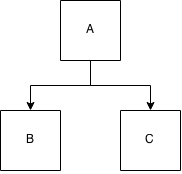
\includegraphics{pictures/cp_system.png}
  \caption{CP-system with a single master node and two slaves}
\label{cpimage}
\end{figure}

CP-systems endorse data consistency over availability. In practice this means
that when a network between two or more database nodes malfunctions, the
system should stop handling both, read and write requests from clients and wait
until the network is healed. Failure to do so might bring the systems into an
inconsistent state, where nodes of the system have different view of the same
datum. Consider figure~\ref{cpimage} that shows a CP-system consisting of a
single master node \(A\) and two slaves \(B\) and \(C\). Clients are able to
read from all of the nodes, but only node \(A\) accepts writes. After a
successful write, \(A\) replicates the write to the slave nodes. If the
connection between \(A\) and \(B\) fails, the system is partitioned into two
sets, one containing \(A\) and \(C\), and other containing only \(B\). Now if
the client first writes a new document to \(A\) and then tries to read it from
both \(B\) and \(C\), what happens is that \(C\) correctly returns the written
document, but \(B\) reports that the document can not be found. This happens
because master \(A\) was not able to replicate the new write to node \(B\)
because the network between the nodes was down. Because now \(B\) and \(C\) have
a different view of the same datum, the system can not be considered as
CP-system anymore. The situation can be fixed by not accepting a write from the
client, when the master node detects that it is not able to replicate the writes
to all nodes. 

As in the example, a common way to model CP-systems is a master/slave
architecture, where one node at a time acts as a master and other nodes are
slaves. To achieve consistency, only master is able to accept write requests and
depending on the architecture, slaves might be able to accept read requests. If
slaves handle the read requests, blabla eventual consistency next

\subsection{AP-systems}

\missingfigure{AP-system}
